\documentclass[10,a4paper]{article}
\usepackage[T2A]{fontenc}
\usepackage[utf8]{inputenc}
%koi8-r]{inputenc}
\usepackage[english,russian]{babel}
\usepackage{amsmath}
\usepackage{amsfonts}
\usepackage{amssymb}
\usepackage[top=1cm,bottom=1cm]{geometry}

% \usepackage{color}
\usepackage[usenames,dvipsnames,svgnames,table]{xcolor}
\usepackage[colorlinks=true, linkcolor=Maroon]{hyperref}
\pagestyle{empty}


\newcommand*{\mc}{}
\def\mc#1#{\mathcoloraux{#1}}
\newcommand*{\mathcoloraux}[3]{%
  \protect\leavevmode
  \begingroup
    \color#1{#2}#3%
  \endgroup
}

\usepackage{wrapfig}


\usepackage{graphicx}
\usepackage{physics}

\usepackage{textcomp}

\usepackage{comment}
\newcommand{\fref}[1]{Рис.~\ref{#1}}
\newcommand{\tref}[1]{Таб.~\ref{#1}}
\newcommand{\eref}[1]{(\ref{#1})}


\renewcommand{\labelenumii}{\arabic{enumii}.}
\renewcommand{\thesubsubsection}{\arabic{subsubsection}}

\usepackage{listings}

\lstset{basicstyle=\footnotesize\ttfamily,breaklines=true}
\lstset{framextopmargin=50pt}
\lstset{language=Pascal,
    keywordstyle=\color{blue},
    commentstyle=\color{magenta},
    numberstyle=\tiny\color{gray},
    stringstyle=\color{orange},
    numbers=left
}

\setcounter{secnumdepth}{6}
\setcounter{tocdepth}{4}

\title{Массивы}

\begin{document}
\section{Массивы}
\subsubsection{Рекурсия}
Повторим предыдущую тему: нарисуйте двоичное дерево,
смотри~рис.~\ref{fig:btree}.
\begin{lstlisting}
procedure btree(x, y, xstep, level: integer);
var
    newy, new_step: integer;
begin
    newy := y + 64;
    if (newy < getmaxy) and (xstep > 0) then
    begin
        new_step := xstep div 2;
        setcolor(level + 1);
        line(x, y, x - xstep, newy);
        line(x, y, x + xstep, newy);
        btree(x - xstep, newy, new_step, level + 1);
        btree(x + xstep, newy, new_step, level + 1)
    end
end;
\end{lstlisting}
\begin{figure}[!ht]
    \begin{centering}
        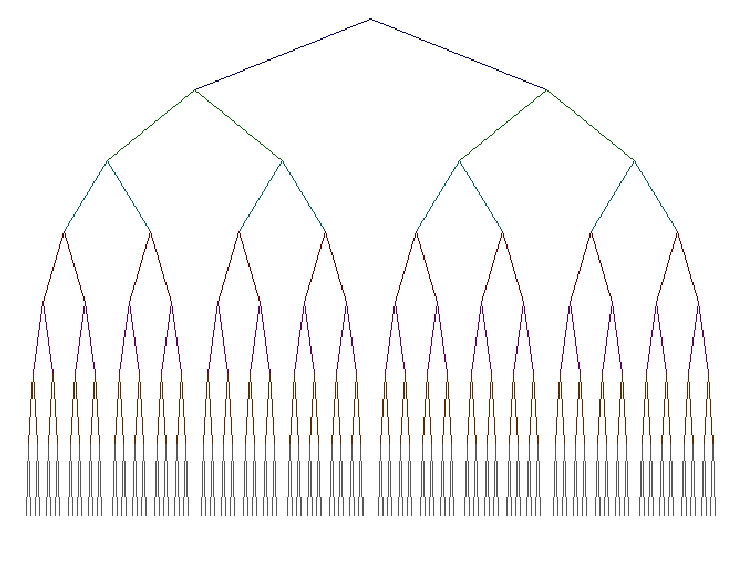
\includegraphics{btree}
        \caption{Двоичное дерево.}
        \label{fig:btree}
    \end{centering}
\end{figure}
\subsubsection{Границы массива}
Что произойдёт, если выйти за границы массива?
\begin{lstlisting}
program boundaries;

var
    i: integer;
    x: integer;
    nums: array [1..10] of integer;
begin
{   nums[-34] := -32; }
    i := 0;
    x := 16;
    writeln('x = ', x);
    { now we do not touch variable j }
    nums[i] := -32;
    writeln('x = ', x);
    readln
end.
\end{lstlisting}
\subsubsection{Случайные числа}
Заполните массив из 24 целых чисел случайным образом от нуля до ста.
\begin{lstlisting}
program fill_random;

var
    nums: array [1..24] of integer;
    i: integer;

begin
    for i := 1 to 24 do
        nums[i] := random(100);
    for i := 1 to 24 do
        writeln('nums [', i, '] = ', nums[i])
end.
\end{lstlisting}
\subsubsection{Максимум}
Найдите максимум в массиве из случайных чисел.
\begin{lstlisting}
function maximum: integer;
var
    i, tmp: integer;
begin
    tmp := 0;
    for i := 1 to 24 do
        if tmp < nums[i] then
            tmp := nums[i];
    maximum := tmp;
end;
\end{lstlisting}
\subsubsection{Минимум}
Найдите минимум в массиве из случайных чисел.
\subsubsection{Поиск элемента}
В массиве из случайных чисел найдите позицию, в которой находится число
\texttt{50}. Если такой позиции нет, напишите \texttt{-1}. Выведите на
экран, сколько раз приходится сравнивать элементы массива.
\begin{lstlisting}
function find(a: integer): integer;
var
    i: integer;
begin
    find := -1;
    for i := 1 to 24 do
    begin
        if a = nums[i] then
        begin
            find := i;
            break
        end
    end 
end;
\end{lstlisting}
\subsubsection{Перестановка}
Напишите процедуру, которая будет переставлять два элемента.
\begin{lstlisting}
procedure perm(i, j: integer);
var
    tmp: integer;
begin
    tmp := nums[i];
    nums[i] := nums[j];
    nums[j] := tmp;
end;
\end{lstlisting}
\subsubsection{Сортировка}
Отсортируйте массив в порядке возрастания. Сколько перестановок
потребовалось?
\begin{lstlisting}
procedure buble;
var
    i, j: integer;
begin
    nperm := 0;
    for i := 1 to 24 do
        for j := i + 1 to 24 do
            if nums[j] < nums[i] then
                perm(i, j);
end;
\end{lstlisting}
\subsubsection{Бинарный поиск}
Сортируйте массив в порядке возрастания.
При сортировке массива сохраните начальные позиции чисел в массиве.
\begin{lstlisting}
function search(a: integer): integer;
label end_search;
var
    curr, step, ostep: integer;
    left, right: integer;
begin
    ncomp := 0;
    search := -1;
    curr := asize div 2;
    step := curr;
    repeat
        if nums[curr] = a then
        begin
            search := inds[curr];
            goto end_search
        end
        else
            if a < nums[curr] then
            begin
                curr := curr - step;
                if curr < 1 then
                    curr := 1;
            end
            else
            begin
                curr := curr + step;
                if curr > asize then
                    curr := asize;
            end;
        ostep := step;
        step := step div 2;
    until step <= 1;
    left := curr - ostep;
    if left < 1 then
        left := 1;
    right := curr + ostep;
    if right > asize then
        right := asize;
    for curr := left to right do
        if a = nums[curr] then
            search := inds[curr];
end_search: ;
end;
\end{lstlisting}
\subsubsection{Стек}
Стек --- это структура данных в виде <<стопки>> однотипных переменных.
Пользователь имеет доступ только до верхнего элемента.
Напишите процедуру \texttt{push(x: integer)}, которая кладёт новый
элемент \texttt{x} в <<стопку>>, и функцию \texttt{pop: integer},
которая возвращает верхний элемент <<стопки>> и возвращает его значение.
\begin{lstlisting}
program stack_program;

const ssize = 128;
var
    stack: array [1..ssize] of integer;
    sp: integer;

procedure init_stack;
begin
    sp := 0;
end;

procedure push(x: integer);
begin
    if sp < ssize then
    begin
        sp := sp + 1;
        stack[sp] := x;
    end
    else
    begin
        writeln('Stack overflow');
        exit;
    end
end;

function pop: integer;
begin
    if sp >= 1 then
    begin
        pop := stack[sp];
        sp := sp - 1;
    end
    else
    begin
        writeln('Stack underflow');
        exit;
    end
end;

var
    i: integer;
    tmp: integer;
begin
    for i := 1 to 5 do begin
        tmp := random(100);
        writeln('push ', tmp, ' on stack');
        push(tmp);
    end;
    for i := 1 to 5 do begin
        writeln('pop  ', pop, ' from stack');
    end
end.
\end{lstlisting}
\end{document}
